% SPDX-License-Identifier: LPPL-1.3c
% Copyright (C) 2026 Christophe Jorssen
% Author and Current Maintainer: Christophe Jorssen <christophe.jorssen@gmail.com>
% LPPL maintenance status: maintained
% This file is part of luafemm. See LICENSE and LICENSES.md for its terms.
\section{Singular sources with dielectric and conductor response}
\label{sec:electric-hybrid}
\index{electrostatics!source correction}
\index{electrostatics!singular sources}

Select |model=source correction| to combine exact singular sources with a
finite-element correction for surrounding dielectrics and voltage- or charge-controlled electrodes.
The common electric field, vector, equipotential and profile interfaces then
use the total solution. The runtime remains entirely in Lua.

There are two physical geometries. In |problem type=planar|, a source node
represents an infinite straight line perpendicular to the drawing, with signed
charge per length in C/m. In |problem type=axisymmetric|, a node on $r=0$
represents one three-dimensional point charge, in C. The meridional drawing
represents a complete revolution. A point away from the axis would describe
neither of these sources and is rejected. General three-dimensional arrays of
point charges near arbitrary conductors are outside this model.

The original |femm/point charge| shape remains the homogeneous Coulomb model
of Section~\ref{sec:electric-charge}. It cannot be placed in this model; use
|femm/electric source| and explicitly choose the appropriate physical strength.
A label such as $+$ is only node text: it does not assign the charge.

\subsection{A line source, a dielectric and a grounded conductor}
The following section is invariant perpendicular to the page. A positive line
charge of $10^{-10}\,\mathrm{C/m}$ lies in air, beside a dielectric slab and a
circular grounded conductor. The faint rectangle is also grounded: it is the
finite computational boundary, not a clipping window or infinity. The dotted
contour $\Gamma$ crosses the dielectric and captures the same solution as the
field drawing. Lengths are in the default centimetre unit.

Start with |mesh size=.2| to keep preparation inexpensive. This controls the
regular correction, while the source field itself is evaluated analytically.
Declare all regions, electrodes and sources before drawing the field or
capturing a profile. The first evaluation solves the model and freezes it.
A named picture also solves when it ends. Requesting the mesh alone already
locks the physical declarations. Subsequent ordinary labels are harmless.

\luafemmexamplebegin{electric-source-correction}
\Needspace{16cm}
\begin{codeexample}[width=0pt]
\begin{tikzpicture}[femm/electrostatic={model=source correction,
    xmin=-2.2,xmax=2.2,ymin=-1.5,ymax=1.7,mesh size=.2,
    name=dielectric source},scale=1.1]
  \draw[gray!40] (-2.2,-1.5) rectangle (2.2,1.7);
  \filldraw[fill=blue!8,draw=blue!40,
    femm/electric region={relative permittivity=4}]
    (.15,-.8) rectangle (.7,1.15);
  \filldraw[fill=gray!25,thick,
    femm/electric electrode={name=metal,potential=0}]
    (1.3,-.75) circle[radius=.35];
  \node[femm/electric source={charge per length=1e-10,
    source guard radius=.12,exclusion radius=.22},fill=red!15]
    at (-.8,.2) {$+$};
  \pic[femm/electric={lines per charge=18,step=.06}]
    {femm electric field};
  \pic[femm/electric={levels={.3,.6,1,2,3},contour resolution=40}]
    {femm equipotentials};
  \draw[densely dotted,femm/electric profile={name=dielectric trace,samples=121}]
    (-1.8,.6)--(1.8,.6) node[right] {$\Gamma$};
  \node[above,fill=white,inner sep=1pt] at (.425,1.15) {$\epsilon_r=4$};
  \node[below] at (1.3,-1.1) {$V=0$};
\end{tikzpicture}
\end{codeexample}

The dielectric changes the direction and magnitude of the field. Lines end on
the conductor and on the exterior boundary. The potential remains continuous
across the slab; its slope changes. To display a component of $\mathbf E$ or
$\mathbf D$, change |component=V| in the following plot. Raw correction gradients
jump at triangle faces, so field profiles retain gaps at these faces rather
than joining two one-sided values with a fictitious segment. Potential profiles
remain continuous away from source masks.

\Needspace{10cm}
\begin{codeexample}[width=0pt]
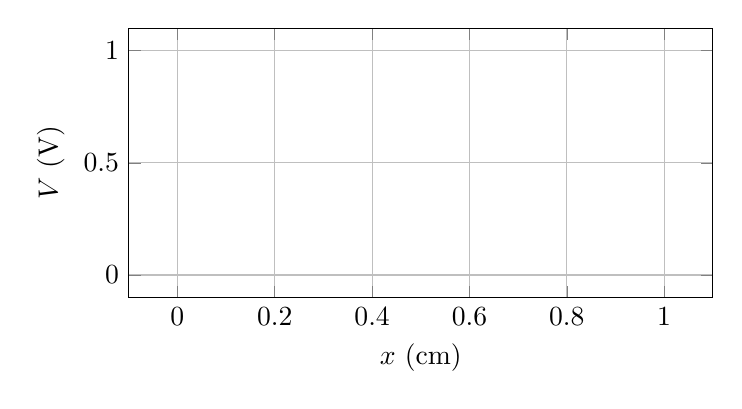
\begin{tikzpicture}
  \begin{axis}[width=9cm,height=5cm,xlabel={$x$ (cm)},
    ylabel={$V$ (V)},grid=major]
    \femmelectricplot[profile=dielectric trace,component=V,
      abscissa=x,plot options={blue,thick,mark=none}]
  \end{axis}
\end{tikzpicture}
\end{codeexample}
\luafemmexampleend{electric-source-correction}

\subsection{An axial point inside a grounded spherical shell}
A charge $q=1\,\mathrm{pC}$ sits at $z=a=0.3\,\mathrm{cm}$ inside a sphere of
radius $R=1.2\,\mathrm{cm}$. Draw the right-hand meridian as an open arc and
use |interior=dielectric|: the interior contains the field, rather than solid
metal. Revolving the arc about $r=0$ gives the entire shell. The computational
axis has its regular symmetry condition; it is not a zero-potential electrode.
The small negative-$r$ part of the source glyph is purely typographical.

\luafemmexamplebegin{electric-source-axis}
\Needspace{16cm}
\begin{codeexample}[width=0pt]
\begin{tikzpicture}[femm/electrostatic={model=source correction,
    problem type=axisymmetric,xmin=0,xmax=1.6,ymin=-1.6,ymax=1.6,
    mesh size=.15,name=spherical source},scale=1.4]
  \draw[gray!40] (0,-1.6) rectangle (1.6,1.6);
  \draw[dash dot,gray] (0,-1.6)--(0,1.6) node[above] {$z$};
  \draw[very thick,blue!60!black,
    femm/electric electrode={potential=0,interior=dielectric}]
    (0,-1.2) arc[start angle=-90,end angle=90,radius=1.2];
  \node[femm/electric source={kind=axis point charge,charge=1e-12,
    source guard radius=.1,exclusion radius=.22},fill=red!15]
    at (0,.3) {$+$};
  \pic[femm/electric={lines per charge=12,step=.04}]
    {femm electric field};
  \pic[femm/electric={levels={.1,.3,.6,1,2},contour resolution=40}]
    {femm equipotentials};
  \draw[densely dotted,femm/electric profile={name=sphere trace,samples=101}]
    (.15,0)--(1.1,0) node[above left] {$\Gamma$};
  \node[above right] at (.85,.85) {$V=0$};
\end{tikzpicture}
\end{codeexample}

The independent image solution inside the sphere has an image $q'=-qR/a$
at $z'=R^2/a$. Neither the image nor its position needs to be declared in the
numerical model: the grounded arc causes the correction. On $\Gamma$, where
$z=0$, the exact potential is
\[
 V(r,0)=\frac{q}{4\pi\epsilon_0}
 \left[\frac{1}{\sqrt{r^2+a^2}}-
       \frac{R/a}{\sqrt{r^2+(R^2/a)^2}}\right].
\]
The formula below uses centimetres on the horizontal axis and volts vertically.
The numerical result also approximates the circle by constrained straight
segments; reducing |curve tolerance| and |mesh size| tests this error.

\Needspace{10cm}
\begin{codeexample}[width=0pt]
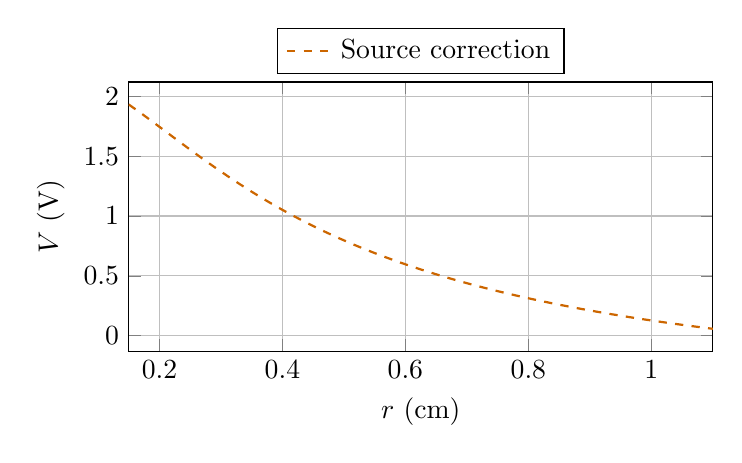
\begin{tikzpicture}
  \begin{axis}[width=9cm,height=5cm,xmin=.15,xmax=1.1,
    xlabel={$r$ (cm)},ylabel={$V$ (V)},grid=major,
    legend style={at={(.5,1.03)},anchor=south}]
    \femmelectricplot[profile=sphere trace,component=V,abscissa=r,
      plot options={blue,thick,mark=none}]
    \addlegendentry{Source correction}
    \addplot[orange!80!black,dashed,thick,domain=.15:1.1,samples=81]
      {.898755179226*(1/sqrt(x*x+.09)-4/sqrt(x*x+23.04))};
    \addlegendentry{Spherical image formula}
  \end{axis}
\end{tikzpicture}
\end{codeexample}
\luafemmexampleend{electric-source-axis}

\subsection{Source nodes and physical keys}
\label{sec:electric-source-keys}
All lengths below use |/femm/electrostatic/length unit|, initially |cm|.
Strengths always use SI and are unaffected by coordinate scaling. Node-local
shifts and rotations transform the physical centre; a root picture transform
changes the presentation of the whole model. Node anchors and |minimum size|
change the glyph, not a physical charge radius. The source has no finite core.

\begin{key}{/tikz/femm/electric source=\meta{options} (default \normalfont empty)}
Apply to a node before any meshing or evaluation. Selects the circle shape
|femm electric source| and the existing |femm charge| drawing style, and processes
\meta{options} in |/femm/electric source|. The final transformed centre is
registered once. Standard circle anchors, TikZ text, fills, borders and styles
are available. Immediate node placement is required; matrix and late-positioned
nodes fail rather than register a provisional position. This key needs an
active |model=source correction| picture. The numerical source remains active
when the glyph is hidden by |opacity=0| or omitted from the bounding box by
|overlay|. Ordinary TeX grouping applies to its options.
\end{key}
\begin{key}{/femm/electric source/kind=\meta{choice} (initially line charge)}
|line charge| requires a planar problem and |charge per length|.
|axis point charge| requires an axisymmetric problem, $r=0$, and |charge|.
The existing physical boundary-snap tolerance absorbs TeX rounding at the axis;
it does not permit an off-axis source. The kind is never inferred from the
strength or changed automatically when the problem type changes.
\end{key}
\begin{key}{/femm/electric source/charge per length=\meta{number} (initially \normalfont empty)}
Required finite signed line strength $\lambda$ in C/m for |kind=line charge|.
Zero is allowed. Supplying |charge| as well is an error, even if it is zero.
\end{key}
\begin{key}{/femm/electric source/charge=\meta{number} (initially \normalfont empty)}
Required finite signed point strength $q$ in C for |kind=axis point charge|.
Zero is allowed. Supplying |charge per length| as well is an error. Strengths
and radii accept PGF numerical expressions; text is transported safely to Lua.
Coincident sources add before evaluation. Exact cancellation removes the
singularity and its exclusion; otherwise the largest coincident guard and
exclusion radii are retained. There is no distance-based merging of distinct
physical sources.
\end{key}
\begin{key}{/femm/electric source/source guard radius=\meta{positive number} (initially .1)}
Radius of a homogeneous neighbourhood in model units. The complete ball must
lie in the background scalar dielectric, strictly clear of all conductor
surfaces, contrasting dielectrics and exterior voltage boundaries. For an
axial point its meridional half-ball may touch $r=0$. The meshed geometry is
checked, including thin electrodes; intersections cause an explicit error.
The guard certifies that the contrast integral has no source singularity.
It neither removes material, changes the physical kernel, nor inserts a mesh
hole. A smaller positive guard can permit a closer interface, but requires
independent quadrature and mesh checks.
\end{key}
\begin{key}{/femm/electric source/exclusion radius=\meta{positive number} (initially .22)}
Radius of the visual and profile exclusion, in model units, independent of the
guard. Lines and vector arrows stay outside it; contours conservatively omit
subtriangles touching it. Profiles crossing it fail by default; the common
|outside=nan| policy inserts gaps, including a crossing hidden between requested
sample positions. The radius does not soften the kernel or alter the solve.
It need not equal the drawn node size or the guard. Excessively large masks
can hide nearby interfaces or entire field lines.
\end{key}

The common |relative permittivity| and named dielectric |material| choices set
the homogeneous reference medium. Region paths may replace it with another
positive scalar permittivity. Tensor entries must describe an isotropic medium;
rotated anisotropy is not supported here. A source must stay in the reference
medium even if another region elsewhere has the same shape or name.

The existing |reference radius| has a specific meaning for planar source
correction: empty selects $d_0=1$ model unit in the logarithmic source kernel.
An explicit positive value changes the split $V_s+u$ but not the total solution
with the same prescribed voltages. It is rejected in axisymmetry. Set physical
voltages with |boundary potential| and electrode |potential|, not with this
arbitrary logarithmic reference or the classical |reference potential| key.

\begin{key}{/femm/electrostatic/source quadrature tolerance=\meta{number} (initially .000001)}
Relative local tolerance, strictly between zero and one, for the smooth source
contrast load. Positive Gauss--Duffy rules compare a triangle with its four
children using an absolute-integrand scale, so cancellation of a vector
component does not create a false convergence test. This is a quadrature
estimate, not a certified field error or a substitute for mesh refinement.
Set before the picture begins. It is owned by a saved model; a restoration
cannot override it. Cells with no dielectric contrast need no volume source quadrature.
Boundary terms and mixed-flux measurements use the same relative tolerance.
\end{key}
\begin{key}{/femm/electrostatic/maximum source quadrature depth=\meta{integer} (initially 8)}
Adaptive subdivision depth, from 1 to 12, for contrast and source-boundary loads. Exhaustion
before the tolerance is met fails explicitly. It has the same physical-model
scope as the quadrature tolerance.
\end{key}
\begin{key}{/femm/electrostatic/maximum source quadrature cells=\meta{integer} (initially 250000)}
Budget from 1 to 2000000 for all evaluated quadrature cells in one solve,
including trial child rules and the reported mixed-boundary flux. A volume
cell uses sixteen kernel evaluations; a boundary rule uses four. An energy
baseline or matrix column has its own solve budget.
Exhaustion fails before a solved snapshot is saved. Increase this only after
checking the geometry, source guard and requested tolerance.
\end{key}

\subsection{Drawing controls, profiles and refinement}
\label{sec:electric-source-views}
The common |femm/electric| options and drawing styles apply. Automatic field
seeds surround sources selected by |seed sign|; |lines per charge| controls
their number. An axial source uses the positive-$r$ semicircle. Line density
is illustrative and is not a calibrated electric flux. With no active sources,
provide explicit seeds or a seed contour to draw an electrode-driven field.
The |step|, |tolerance|, length and step budgets control numerical tracing of
the total field. Lines stop at electrodes, exclusion disks, view/domain bounds
and field nulls; inconsistent one-sided directions in a coarse raw correction
can also stop a line at a mesh face. Refine the mesh before interpreting such
an endpoint as a physical feature.

Equipotentials evaluate the total potential inside dielectric triangles.
The common |contour resolution| selects a target subtriangle edge length from
the view width; |levels| gives explicit voltages or |count| selects levels
from sampled eligible potentials. The following additional keys affect only
source-correction equipotentials, with the common view/pic scope. They do not
modify a saved physical model.

\begin{key}{/femm/electric/contour tolerance=\meta{positive number} (initially .002)}
Relative potential-deviation threshold for adaptive contour subdivision.
Midpoints and centroids are compared with affine interpolation and normalized
by the eligible sampled potential range. This supplements |contour resolution|;
it is not a solver residual, an error bound on the whole contour, or a tolerance
in volts. A nearly constant potential may need a larger value. Roots on leaf
edges are evaluated from the nonlinear total potential. Joined straight
segments approximate the curve between those roots.
\end{key}
\begin{key}{/femm/electric/maximum contour depth=\meta{integer} (initially 8)}
Maximum subtriangle depth, from 1 to 14. Failure to reach the requested size
and potential-deviation criteria is an error. No partial contour drawing is
returned as if complete.
\end{key}
\begin{key}{/femm/electric/maximum contour cells=\meta{integer} (initially 250000)}
Subdivision budget from 1 to 2000000, shared by all levels in one contour view.
It counts visited subtriangles, including discarded or subdivided cells.
Contours never interpolate through a solid electrode or a source mask.
\end{key}

Normal PGF styles can keep the numerical policy separate from the source glyph.
This smaller variant uses tighter contrast quadrature and finer contour drawing.
Its deliberately coarse field mesh is still suitable for a first layout.

\Needspace{12cm}
\begin{codeexample}[width=0pt]
\tikzset{
  source model/.style={femm/electrostatic={model=source correction,
    xmin=-1.5,xmax=1.5,ymin=-1,ymax=1,mesh size=.3,
    source quadrature tolerance=1e-7,
    maximum source quadrature depth=9,
    maximum source quadrature cells=300000}},
  fine electric contours/.style={femm/electric={levels={.5,1,2},
    contour resolution=45,contour tolerance=.001,
    maximum contour depth=9,maximum contour cells=300000}},
  positive line/.style={femm/electric source={charge per length=1e-10,
    source guard radius=.12,exclusion radius=.22},fill=red!15}}
\begin{tikzpicture}[source model]
  \filldraw[fill=blue!8,femm/electric region={relative permittivity=3}]
    (.3,-1) rectangle (1.5,1);
  \node[positive line] at (-.5,0) {$+$};
  \pic {femm electric field};
  \pic[fine electric contours] {femm equipotentials};
\end{tikzpicture}
\end{codeexample}

Before preparing a final quantitative figure, vary four controls separately:
\begin{enumerate}
\item Reduce |mesh size| at fixed physical domain and source data; compare the
      desired potential or field profile. Refine curved path flattening too.
\item Move the exterior boundary while holding the local mesh resolution;
      compare the observable again. A finite grounded rectangle can dominate
      a nominally open-field problem even with many triangles.
\item Tighten |source quadrature tolerance| until the same result stabilizes.
      This matters particularly near a high-contrast dielectric interface.
\item Refine the drawing |step| and |contour resolution| and their tolerances.
      These alter visual approximation, not the physical solution.
\end{enumerate}
The named snapshot owns sources, guards, permittivities, geometry, correction
coefficients and solver settings. Profiles likewise own their sampled model.
Restoring with |snapshot=...| reuses that state; changing view options, line
styles or the root display transform does not require a new solve. Numerical
components are in SI: $V$ in volts, $E$ in V/m, $D$ in C/m$^2$; |Er|, |Ez|,
|Dr|, |Dz|, |r| and |z| aliases apply only to axial profiles.

\subsection{Numerical meaning and limits}
The source/correction weak form is given in Section~\ref{sec:electric-correction}.
Only $u$ is represented by continuous piecewise affine finite elements.
The total field is $-\nabla V_s-\nabla u$, evaluated at the requested position;
it varies within a triangle. A total Dirichlet value $g$ is imposed as
$u_i=g-V_s(x_i)$ at boundary nodes. Between nodes its total trace has the
interpolation error of this correction. Curved conductors additionally have
polygonal geometry error. Mesh and curve refinement address both effects.
The dielectric flux-continuity condition is satisfied weakly, not pointwise by
each raw triangle gradient.

This provider accepts positive symmetric tensor contrasts outside the source
guards, voltage or total-charge conductors, the regular axis, and the exterior
conditions of Section~\ref{sec:electric-extended}. The reference background
and every guard remain homogeneous and isotropic. A rotated tensor touching
the regular axis must have zero radial--axial coupling. Solid electrodes return
their solved total potential and zero field inside. Additional volume, surface
and native point-property loads remain rejected: all prescribed singular sources
must belong to the explicit source list. Use the ordinary finite-element
provider for nonsingular volume and sheet sources.

|\femmelectricvalue| supports mesh/solver counts, electrode |voltage| and
|charge|, global source |charge|, |charge balance| and |periodic flux|, with the
same total/per-length conventions as the ordinary FE provider. The balance is
source charge plus conductor reactions minus outward displacement flux. A small
balance error checks assembly and constraint consistency; it does not bound the
error of the local field or a force. Ordinary |energy|, |boundary energy| and
|total energy| remain unavailable. The finite interaction quantity below is a
separate definition, not an estimate of divergent total self-energy.

Native |.fee| and |.res| export reject this model before writing a file. Their
ordinary nodal-potential representation cannot retain the analytical kernel and
its exact off-node field. Replacing the kernel by nodal samples would change the
problem and can even place an infinite value on a source node. The in-memory
snapshot is available; no hybrid disk-restart format or silent nodal
approximation is implied.

\subsection{Floating conductors, tensors and charge offsets}
\label{sec:electric-source-response}
Reuse the electrode, dielectric and matrix key families from
Section~\ref{sec:electric-extended}. No second set of physical keys is needed.
A floating conductor is declared with |condition=charge|; its omitted charge
is zero. In a planar picture an explicit conductor |charge| is in C over the
specified |depth|, whereas a source node's |charge per length| is in C/m.
The distinction matters when comparing their balance.

Here a neutral metal screen responds to a line charge between two voltage
ports. The rotated dielectric has principal relative permittivities 2 and 5.
The upper and lower sides are insulating; they are physical boundaries of
this cell. The source's guard lies entirely in the isotropic air background.
As always, finish physical declarations before the first field pic, profile,
force or matrix. Obtain values from the named, solved picture afterwards.

\luafemmexamplebegin{electric-source-response}
\Needspace{22cm}
\begin{codeexample}[width=0pt]
\tikzset{neutral metal/.style={fill=gray!20,thick,
    femm/electric electrode={name=screen,condition=charge}},
  source port/.style={very thick,blue!60!black}}
\begin{tikzpicture}[femm/electrostatic={model=source correction,
    xmin=-1.5,xmax=1.5,ymin=-1,ymax=1,outer boundary=insulated,
    mesh size=.15,name=source ports},scale=1.8]
  \draw[source port,femm/electric electrode={name=left,potential=2}]
    (-1.5,-1)--(-1.5,1);
  \draw[source port,femm/electric electrode={name=right,potential=0}]
    (1.5,-1)--(1.5,1);
  \filldraw[neutral metal] (.15,-.5) rectangle (.4,.5);
  \filldraw[fill=blue!8,draw=blue!40,femm/electric region={
      relative permittivity x=2,relative permittivity y=5,
      material angle=30}] (.7,-.6) rectangle (1.15,.6);
  \node[femm/electric source={charge per length=1e-10},fill=red!15]
    at (-.65,0) {$+$};
  \pic[femm/electric={lines per charge=16,step=.04}]
    {femm electric field};
  \pic[femm/electric={levels={.5,1,2,3}}] {femm equipotentials};
  \node[above] at (-1.5,1) {$2$ V};
  \node[above] at (1.5,1) {$0$ V};
  \node[above,fill=white,inner sep=1pt] at (.275,.5) {$Q_s=0$};
  \node[below,fill=white,inner sep=1pt] at (.925,-.6) {$\epsilon_1=2,\ \epsilon_2=5$};
\end{tikzpicture}

$V_s=\femmelectricvalue[model=source ports,electrode=screen,
    quantity=voltage]$ V.
\end{codeexample}

The matrix uses the same mesh and floating constraint. Its offset now includes
the singular source. Each unit-column solve removes the independent source and
retains zero incremental charge on the screen. Thus $Q_i=q_i^{(0)}+\sum_jC_{ij}V_j$
reconstructs the original operating charges. The two offset charges sum to
$-\lambda$ per unit length in this insulating cell, since the screen is neutral.
The negative off-diagonal entry is the conventional Maxwell coefficient.

\Needspace{16cm}
\begin{codeexample}[width=0pt]
\femmelectricmatrix[name=source capacitance,model=source ports,
    electrodes={left,right},normalization=per length]
$q_L^{(0)}/L=\femmelectricmatrixvalue[matrix=source capacitance,
    row=left,quantity=offset charge]$ C/m,
\quad
$q_R^{(0)}/L=\femmelectricmatrixvalue[matrix=source capacitance,
    row=right,quantity=offset charge]$ C/m.
\end{codeexample}

\Needspace{12cm}
\begin{codeexample}[width=0pt]
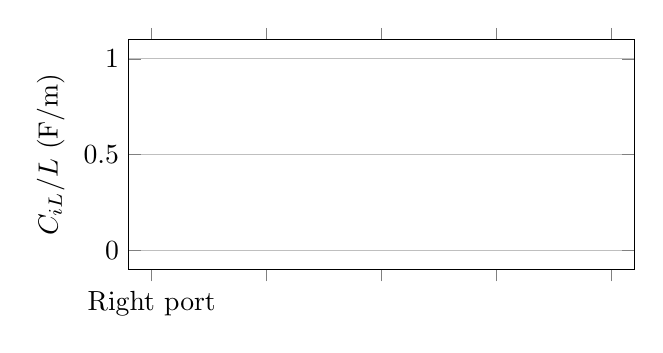
\begin{tikzpicture}
  \begin{axis}[width=8cm,height=4.5cm,ybar,
      xtick={1,2},xticklabels={Left port,Right port},
      ylabel={$C_{iL}/L$ (F/m)},ymajorgrids,
      enlarge x limits=.6,bar width=16pt]
    \femmelectricmatrixplot[matrix=source capacitance,column=left,
      plot options={fill=blue!25,draw=blue!60!black}]
  \end{axis}
\end{tikzpicture}
\end{codeexample}
\luafemmexampleend{electric-source-response}

For a floating or paired boundary, it is the \emph{total} nodal voltage which
obeys the constraint. Internally $u_i=s_i U+o_i$, where $s_i=\pm1$ and
$o_i=-V_s(x_i)$ on constrained nodes. This allows a nonconstant correction on
an equipotential conductor. The singular kernel is never evaluated at an
unconstrained interior source vertex during this reduction.

The tensor contrast load is
$\int(\boldsymbol\epsilon-\epsilon_b I)\mathbf E_s\cdot\nabla w$.
On an active dielectric boundary, including a solid-conductor hole, the load
also contains $\int\epsilon_b\mathbf E_s\cdot\mathbf n\,w$.
These reference-flux terms make the constrained equation residual the
\emph{total} conductor charge. Opposite traces cancel on a thin internal
conductor. Integrating only the correction field would miss induced charge.

\subsection{Natural, mixed and periodic boundaries}
All existing electric boundary choices apply, with unchanged units and path
rules. An insulating side imposes total $D_n=0$. For a mixed side,
$D_n=cV+g$ gives the additional correction load $-\int(cV_s+g)w$ and stiffness
$\int cuw$. The reported exterior flux evaluates $c(V_s+u)+g$ along each edge;
it does not interpolate total potential from its endpoint samples.
Periodic and antiperiodic pairs impose total $V_2=\pm V_1$ at matched nodes.
Their reference fluxes enter the weak equations as well. In axisymmetry only
axial translations are admissible. These are repeated-cell boundary conditions,
not a claim that the free-space source kernel alone is periodic.

A purely insulating or periodic cell still needs a voltage reference or a
positive mixed coefficient. A compatible antiperiodic constraint removes the
constant mode. No automatic gauge or compensating background charge is added.

\Needspace{14cm}
\begin{codeexample}[width=0pt]
\begin{tikzpicture}[femm/electrostatic={model=source correction,
    xmin=-1,xmax=1,ymin=-1,ymax=1,mesh size=.2},scale=1.4]
  \draw[thick,femm/electric boundary={condition=mixed,
      coefficient=8.8541878128e-10}] (1,-1)--(1,1);
  \path[femm/electric boundary={condition=periodic,pair=vertical}]
    (-1,-1)--(1,-1);
  \path[femm/electric boundary={condition=periodic,pair=vertical}]
    (-1,1)--(1,1);
  \node[femm/electric source={charge per length=1e-10}]
    at (-.3,0) {$+$};
  \pic[femm/electric={lines per charge=12}] {femm electric field};
  \pic[femm/electric={levels={.5,1,2}}] {femm equipotentials};
\end{tikzpicture}
\end{codeexample}
The left side retains the default zero potential. The upper and lower sides
are identified; the right side has a capacitive termination. Field lines stop
at the cell boundary rather than automatically continuing in another cell.

\subsection{Finite source interaction energy}
\label{sec:electric-source-energy}
Subtracting the homogeneous self-kernel defines a finite charging work for
linear media and fixed external data. Let $V_{\rm ext}$ be the source-free
solution with the same applied voltages, floating charges and boundary data;
let $u$ be the correction of the actual source problem. We report
\[
 W_{\rm int}=\sum_i\frac{q_i}{2}
       [u(x_i)+V_{\rm ext}(x_i)]
       +\sum_{i>j}q_i V_{s,j}(x_i).
\]
In a planar problem replace $q_i$ by $\lambda_i$ to obtain energy per length.
The direct source pairs are counted once; self-kernels are never evaluated.
The induced response contributes one half, while an applied external field
contributes once, because it is already present in $u$. This is the extra
source charging work at fixed external data. It excludes both divergent
source self-energy and the energy of the source-free capacitor.

\begin{key}{/femm/electric value/quantity=source interaction energy}
Whole-model finite interaction energy in J, only for |model=source correction|.
Use |\femmelectricvalue| after declarations, optionally selecting |model| by
snapshot name. The usual quantity default remains |charge|. No |electrode|
selector is allowed. Planar values include |depth|; axisymmetric values cover
the full revolution. The first request solves a source-free baseline on the
same mesh and caches the result in that owned state. No source mask enters
this calculation.
\end{key}
\begin{key}{/femm/electric value/quantity=source interaction energy per length}
The same finite quantity in J/m for a planar problem. Rejected in axisymmetry.
Its numerical value depends on the declared logarithmic |reference radius|
by a position-independent constant; its position derivative does not.
Never compare absolute planar interaction energies computed with different
reference conventions. The default reference radius is one model length unit.
\end{key}

\subsection{Force on an enclosed singular source}
\label{sec:electric-source-force}
The existing |femm/electric force| path now integrates the nonlinear total
Maxwell stress. A contour may enclose sources, conductors and anisotropic
objects, but the contour itself must stay in a homogeneous isotropic dielectric
and avoid sources and material/electrode contacts. It measures the resultant
on everything enclosed, not an automatically selected object's force.
A drawing exclusion disk is ignored by this physical integral. Contact with
an actual singular centre fails. A regular-axis closure has zero revolved
area and may pass through an axial source.

\begin{key}{/femm/electric force/quadrature tolerance=\meta{positive number} (initially .000001)}
Relative tolerance less than one for adaptive Gauss integration of each total
stress component along a hybrid contour. Each component uses its own
absolute-integrand scale, so cancellation does not set a zero tolerance.
Path-local, or supplied through a normal TikZ style. This is independent of
|curve tolerance| and |mesh size|; it does not certify physical force accuracy.
Ordinary FE contours use their exact piecewise-constant-field integrals and
ignore this additional quadrature control.
\end{key}
\begin{key}{/femm/electric force/maximum quadrature depth=\meta{integer} (initially 10)}
Maximum adaptive bisection depth from 1 to 16 on each triangle-cut contour
piece. Exhaustion fails without replacing a previously named force result.
Same path-local scope as the tolerance.
\end{key}
\begin{key}{/femm/electric force/maximum quadrature cells=\meta{integer} (initially 250000)}
Shared budget from 1 to 2000000 four-point Gauss rules for one hybrid force
measurement, including trial child rules. Exhaustion is an error. Increasing
this budget cannot correct a contour touching a physical singularity.
\end{key}

A line charge at $a=0.3R$ inside a grounded circular shell is attracted towards
the nearer wall. The section is invariant along the line, with $R=1$ cm and
$\lambda=10^{-10}$ C/m. The dashed green rectangle encloses only the source.
The arrow indicates the force direction; its length is illustrative.

\luafemmexamplebegin{electric-source-force}
\Needspace{21cm}
\begin{codeexample}[width=0pt]
\begin{tikzpicture}[femm/electrostatic={model=source correction,
    xmin=-1.6,xmax=1.6,ymin=-1.6,ymax=1.6,
    mesh size=.1,name=source shell},scale=2]
  \draw[very thick,femm/electric electrode={name=shell,
      potential=0,interior=dielectric,curve tolerance=.002}]
    (0,0) circle[radius=1];
  \node[femm/electric source={charge per length=1e-10,
      exclusion radius=.15},fill=red!15] at (.3,0) {$+$};
  \pic[femm/electric={lines per charge=16,step=.04}]
    {femm electric field};
  \draw[green!40!black,dashed,femm/electric force={name=source force,
      quadrature tolerance=1e-7,maximum quadrature depth=12,
      maximum quadrature cells=300000}]
    (.05,-.25) rectangle (.55,.25);
  \draw[densely dotted,femm/electric profile={name=shell trace,samples=101}]
    (-.85,.4)--(.85,.4);
  \draw[->,red!70!black,thick] (.3,0)--(.7,0) node[above] {$F_x$};
  \node[above] at (0,1) {$V=0$};
\end{tikzpicture}

$F_x/L=\femmelectricforcevalue[force=source force,
    quantity=Fx per length]$ N/m,
\quad
$W_{\rm int}/L=\femmelectricvalue[model=source shell,
    quantity=source interaction energy per length]$ J/m.
\end{codeexample}

The independent image solution gives
\[
 \frac{F_x}{L}=\frac{\lambda^2}{2\pi\epsilon_b}
               \frac{a}{R^2-a^2},\qquad
 \frac{W_{\rm int}}{L}=\frac{\lambda^2}{4\pi\epsilon_b}
               \log\frac{R^2-a^2}{R d_0}.
\]
For the displayed values and default $d_0=1$ cm, these are approximately
$5.926\times10^{-9}$ N/m and $-8.476\times10^{-12}$ J/m.
The plotted trace stays away from the source and compares total potential
with the exact image expression. The image lies at $R^2/a$ outside the shell;
its field is only an independent reference, not an extra numerical source.

\Needspace{14cm}
\begin{codeexample}[width=0pt]
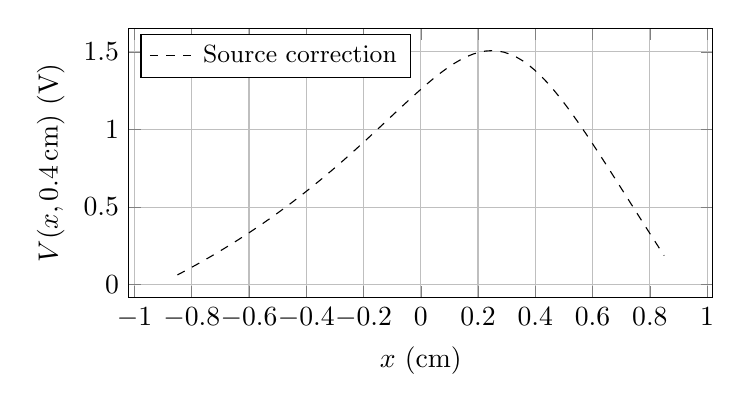
\begin{tikzpicture}
  \begin{axis}[width=9cm,height=5cm,xlabel={$x$ (cm)},
      ylabel={$V(x,0.4\,\mathrm{cm})$ (V)},grid=major,
      legend style={at={(.02,.98)},anchor=north west,font=\small}]
    \femmelectricplot[profile=shell trace,component=V,abscissa=x,
      plot options={blue,thick,mark=none}]
    \addlegendentry{Source correction}
    \addplot[black,dashed,domain=-.85:.85,samples=80]
      {1e-10/(2*pi*8.8541878128e-12)*
       ln(.3*sqrt(((x-1/.3)^2+.4^2)/((x-.3)^2+.4^2)))};
    \addlegendentry{Exact image solution}
  \end{axis}
\end{tikzpicture}
\end{codeexample}
\luafemmexampleend{electric-source-force}

For an axial point inside a grounded sphere, use the meridional geometry of
the preceding spherical example, a closed meridional force contour and
|quantity=Fz|. Its regular-axis closing segment contributes no surface traction.
At axial offset $a$, the exact references are
$F_z=q^2Ra/[4\pi\epsilon_b(R^2-a^2)^2]$ and
$W_{\rm int}=-q^2R/[8\pi\epsilon_b(R^2-a^2)]$.

Refine the field mesh and curved shell together, move the stress contour, and
compare $-\mathrm dW_{\rm int}/\mathrm da$ with the measured force. Piecewise
affine evaluation of the correction at a source and discrete boundary traces
introduce different finite-mesh errors; these two measurements are not exactly
equal on a coarse mesh. A good linear residual, balance or quadrature tolerance
alone is insufficient. No weighted-volume stress, electrostriction or stress
inside an anisotropic medium is supplied by this contour method.
